\documentclass[conference]{IEEEtran}
\IEEEoverridecommandlockouts
\usepackage{cite}
\usepackage{amsmath,amssymb}
\usepackage{graphicx}
\usepackage{booktabs}
\usepackage{url}
\usepackage{tikz}
\graphicspath{{paper/figures/x_readcost/}}
% Generated by x_readcost_paper_tables.py; do not edit.
\newcommand{\HOneP}{7.86\times10^{-9}}
\newcommand{\CampaignSuccess}{519}
\newcommand{\DriftD}{0.979}
\newcommand{\DriftLog}{0.021}
\newcommand{\SensitivityW}{6}
\newcommand{\SensitivityR}{11}

% Generated by x_readcost_paper_tables.py; do not edit.
\gdef\TblArmsRows{%
Memory-tier search under \texttt{Mu.RLock} & yes & yes & yes \\
Reader SSTable I/O under \texttt{Mu.RLock} & yes & no & no \\
Disk-reader lifetime & lock & table leases & set pin \\
Per-read lifetime synchronization & \texttt{Mu} & atomic leases & \texttt{snapshotMu} \\
New set descriptor on publication & no & no & yes \\
Conflict check and WAL sync under \texttt{Mu.Lock} & yes & yes & yes \\
Exclusive acquisitions per successful commit & 2 & 2 & 2 \\
}%

% Generated by x_readcost_paper_tables.py; do not edit.
\gdef\TblXOneRows{%
4 & 0 & 13.6 & 929 & 940 & 978 & 0.988 [0.896, 1.089] & 7{,}468 & 6{,}258 & 6{,}482 & 1.193 [1.089, 1.308] \\
4 & 20\,\(\mu\)s & 33.6 & 878 & 948 & 961 & 0.926 [0.881, 0.974] & 7{,}035 & 4{,}844 & 4{,}909 & 1.452 [1.380, 1.528] \\
4 & 200\,\(\mu\)s & 163 & 615 & 811 & 813 & 0.758 [0.725, 0.793] & 4{,}932 & 4{,}154 & 4{,}161 & 1.187 [1.136, 1.241] \\
4 & 2 ms & 1{,}885 & 130 & 359 & 352 & 0.361 [0.354, 0.368] & 1{,}039 & 1{,}434 & 1{,}408 & 0.725 [0.710, 0.739] \\
4 & legacy scan & 124{,}853 & 2.6 & 613 & 617 & 0.004250 [0.004049, 0.004461] & 21.2 & 43.3 & 43.3 & 0.489 [0.468, 0.511] \\
\midrule
16 & 0 & 21.2 & 856 & 914 & 909 & 0.937 [0.884, 0.993] & 27{,}538 & 25{,}101 & 24{,}972 & 1.097 [1.041, 1.156] \\
16 & 20\,\(\mu\)s & 39.3 & 830 & 880 & 899 & 0.944 [0.887, 1.004] & 26{,}668 & 18{,}620 & 18{,}966 & 1.432 [1.350, 1.519] \\
16 & 200\,\(\mu\)s & 173 & 545 & 773 & 785 & 0.705 [0.676, 0.736] & 17{,}507 & 16{,}017 & 16{,}256 & 1.093 [1.048, 1.140] \\
16 & 2 ms & 1{,}915 & 111 & 358 & 352 & 0.311 [0.305, 0.316] & 3{,}557 & 5{,}693 & 5{,}617 & 0.625 [0.614, 0.636] \\
16 & legacy scan & 430{,}130 & 0.6 & 354 & 355 & 0.001696 [0.001661, 0.001732] & 21.2 & 40.6 & 40.7 & 0.522 [0.501, 0.544] \\
}%

% Generated by x_readcost_paper_tables.py; do not edit.
\gdef\TblMechanismRows{%
X1 & 4 & 0 & 2.009 & 1.664 & 1.657 & 1.077 & 1.130 & 4.9 \\
X1 & 4 & 20\,\(\mu\)s & 2.003 & 1.278 & 1.277 & 1.140 & 1.175 & 3.1 \\
X1 & 4 & 200\,\(\mu\)s & 2.004 & 1.280 & 1.280 & 1.627 & 1.738 & 6.8 \\
X1 & 4 & 2 ms & 2.003 & 0.998 & 1.001 & 7.712 & 7.432 & -3.6 \\
X1 & 4 & legacy & 2.032 & 0.018 & 0.018 & 384.3 & 363.6 & -5.4 \\
\midrule
X1 & 16 & 0 & 2.010 & 1.717 & 1.718 & 1.169 & 1.249 & 6.8 \\
X1 & 16 & 20\,\(\mu\)s & 2.008 & 1.323 & 1.318 & 1.206 & 1.334 & 10.6 \\
X1 & 16 & 200\,\(\mu\)s & 2.006 & 1.295 & 1.294 & 1.835 & 1.978 & 7.8 \\
X1 & 16 & 2 ms & 2.003 & 0.995 & 0.996 & 9.008 & 8.726 & -3.1 \\
X1 & 16 & legacy & 2.209 & 0.007 & 0.007 & 1{,}666.7 & 1{,}437.3 & -13.8 \\
\midrule
X3 & 1 & 0 & 2.009 & 1.080 & 1.081 & -- & -- & -- \\
X3 & 4 & 0 & 2.009 & 1.100 & 1.099 & -- & -- & -- \\
X3 & 16 & 0 & 2.013 & 1.104 & 1.101 & -- & -- & -- \\
}%

% Generated by x_readcost_paper_tables.py; do not edit.
\gdef\TblHTwoPubRows{%
0 & 3.11 [1.54, 6.30] & not equivalent \\
200\,\(\mu\)s & 1.60 [0.51, 4.98] & inconclusive \\
2 ms & 0.53 [0.22, 1.29] & inconclusive \\
legacy scan & 1.08 [0.64, 1.82] & inconclusive \\
}%

% Generated by x_readcost_paper_tables.py; do not edit.
\gdef\TblXTwoRows{%
0 & 318{,}567 & 304{,}721 & 314{,}201 & 20 [20, 20] & 20 [20, 20] & 20 [20, 20] & 247 & 41.60 & 13.37 \\
200\,\(\mu\)s & 75{,}018 & 74{,}678 & 74{,}844 & 20 [20, 20] & 20 [20, 20] & 20 [20, 20] & 450 & 19.33 & 12.10 \\
2 ms & 8{,}437 & 8{,}445 & 8{,}450 & 20 [20, 20] & 20 [20, 20] & 20 [20, 20] & 3{,}886 & 1.51 & 2.83 \\
legacy & 27.6 & 42.7 & 42.7 & 10.5 [9, 11] & 20 [20, 20] & 20 [20, 20] & 1{,}054{,}655 & 1.88 & 1.74 \\
}%

% Generated by x_readcost_paper_tables.py; do not edit.
\gdef\TblXThreeRows{%
1 & W & 697 & 747 & 781 & 0.957 [0.905, 1.012] & [0.910, 0.997] & 65.3/70.1/73.2 \\
1 & R & 1{,}400 & 807 & 844 & 0.956 [0.904, 1.011] & [0.909, 0.997] & -- \\
4 & W & 585 & 702 & 699 & 1.004 [0.963, 1.047] & [0.970, 1.038] & 54.6/65.9/65.5 \\
4 & R & 4{,}703 & 3{,}089 & 3{,}074 & 1.005 [0.964, 1.048] & [0.970, 1.038] & -- \\
16 & W & 415 & 569 & 588 & 0.968 [0.933, 1.004] & [0.938, 0.995] & 38.8/53.2/55.1 \\
16 & R & 13{,}351 & 10{,}050 & 10{,}357 & 0.970 [0.937, 1.005] & [0.941, 0.997] & -- \\
}%

\begin{document}
\raggedbottom
\title{How Long May a Reader Hold the Lock? A Controlled Read-Cost Study of Coarse Locking, Descriptor Leasing, and Immutable Snapshots in an LSM Engine}
\author{\IEEEauthorblockN{V V Ramarathinam Iyer}
\IEEEauthorblockA{\textit{Department of Database Systems, School of Computer Science and Engineering} \\
\textit{Vellore Institute of Technology}, Vellore, Tamil Nadu, India \\
Email: ram.iyer200722@gmail.com}
}

\maketitle
\begin{abstract}
We evaluated coarse locking (A), descriptor leasing (A-min), and immutable reader-set snapshots (B) in a Go LSM engine in a pre-registered 519-trial campaign. All \CampaignSuccess{} trials succeeded on the first attempt. Across ten matched triplets per cell, A's write-throughput ratio to A-min decreased with injected read cost (Page's $L=294$, exact one-sided $p=\HOneP$ at both reader counts). At four readers, the ratio was 0.988 without delay, 0.758 at 200~$\mu$s, and 0.361 at 2~ms. Unexpectedly, A completed more reads than both alternatives through 200~$\mu$s; A/A-min read ratios were 1.19--1.45 at four readers and 1.09--1.43 at sixteen. An exploratory analysis found approximately two reads per reader per commit under A, consistent with two exclusive acquisitions per commit and Go's reader-admission policy. A-min and B met the pre-registered throughput equivalence criterion in all ten write and fourteen read cells; publication lock-wait equivalence was not established. Churn results did not isolate snapshot lifecycle cost. These findings describe this engine and workload, including a writer that retained conflict validation and WAL synchronization under the exclusive lock.
\end{abstract}
\begin{IEEEkeywords}
LSM tree, reader-writer lock, descriptor leasing, immutable snapshots, controlled experiment.
\end{IEEEkeywords}

\section{Introduction}
LSM trees buffer writes in memory and organize persistent data in sorted runs~\cite{oneil1996lsm}. Readers must safely access files while writers and flushers update engine state. Holding a shared manager lock across a lookup provides a simple lifetime guarantee but delays exclusive acquisition. Capturing stable file references before releasing the lock separates lifetime from I/O duration. Performance also depends on the commit path and lock-admission policy.

We compared three arms in one engine: A retained the read lock across SSTable I/O; A-min leased individual table readers; B pinned an immutable reader-set descriptor. We asked how A's write cost changed with read cost (RQ1), whether leasing matched snapshots within a declared margin (RQ2), and how these arms compared during reader-set churn (RQ3). We varied a delay before block reads and retained the defective earlier reader as a separate historical operating point.

The contributions were:
\begin{itemize}
\item A pre-registered, paired, dose-controlled comparison across 17 cells and 519 trials, spanning measured read critical sections from about 14~$\mu$s to 430~ms under A.
\item A write-penalty trend that was small at tens of microseconds and severe at milliseconds, and an unpredicted read-throughput crossover.
\item An exploratory account relating A's read throughput to exclusive acquisitions per commit and Go's reader admission, with reads per reader per commit near 2.00 in every non-legacy cell.
\item Bounded evidence on leasing versus snapshots: throughput equivalence within 10\% in all tested X1/X2 cells, no established publication lock-wait equivalence, and correction of an earlier attribution of churn cost to snapshot lifecycle.
\end{itemize}
The mechanism requires intervention testing; these results do not establish that snapshots are unnecessary in other engines.

\section{Background and Earlier Measurements}
LSM buffering and compaction tradeoffs are surveyed by Luo and Carey~\cite{luo2020}. Reader-set lifetime management preserves files until readers finish. LevelDB and RocksDB provide production reference points~\cite{leveldb,rocksdb}; our arms were implementations in a smaller engine, not measurements of those systems.

The earlier SSTable reader scanned from the target block toward the file's data end, with about four unbuffered syscalls per record and no early stop after passing the target key. This was a defect, now retained only as \texttt{legacy\_scan}. A 960-trial WSL2 campaign comparing A and B and a Windows campaign truncated by a stopping rule (60 of 330 planned trials, 18 complete triplets) used it. They reported B completing 3.3--18.5 times A's writes, and churn throughput B/A of 0.63--0.74 at $r\leq4$. These runs motivated this study; they were not pooled with it and no inference was carried forward. This study supersedes the earlier claims, including the withdrawn $\pm5\%$ equivalence claim and any claim about A-min under churn.

\section{Engine and Synchronization Arms}
\subsection{Storage and point reads}
The memtable used a skip list~\cite{pugh1990}, promotion probability 0.5 and maximum height 32. Internal keys appended an eight-byte big-endian, bitwise-inverted encoding of $(\mathrm{seq}\ll8)\,|\,\mathrm{delete}$ to the user key: 56 effective sequence bits, with the low bit indicating a tombstone. Newer versions sorted first within a user key. Frozen memtables flushed into SSTables.

Data blocks used a 4~KiB flush threshold; a whole record could take a block beyond it. A flat sparse index stored block first keys and offsets, with an index-location footer. The corrected reader checked the cached per-table user-key range, binary-searched the index, and used one \texttt{ReadAt} per visited block. It stopped at a visible version or greater user key. Versions could straddle blocks, requiring further block reads. Open-time range-metadata reads bypassed delay. The path had no application block cache.

\subsection{Lifetime management and commit path}
All arms searched active and frozen memory under \texttt{Mu.RLock}. A retained it through SSTable I/O. A-min copied active reader pointers into reusable scratch storage and took atomic per-table leases in that read-lock interval. It searched outside \texttt{Mu}, then released leases. Superseded readers remained tracked until reclamation. Shutdown closed admission and drained leases on active and retired readers; a timeout returned an error and left leased descriptors open.

B pinned the current immutable reader set under the short manager read lock and \texttt{snapshotMu}, then searched outside both locks. Release also acquired \texttt{snapshotMu}. Publication allocated a new set, assigned \texttt{currentSnapshot} under mutexes, and retired the old set. Drained sets released constituent references; eligible closure and unlinking ran outside \texttt{Mu} and \texttt{snapshotMu}. This was mutex-coordinated management, not a lock-free atomic pointer swap (Table~\ref{tab:arms}).

\begin{table}[t]
\caption{Synchronization arms, audited against the implementation.}
\label{tab:arms}\centering\scriptsize\setlength{\tabcolsep}{2pt}
\begin{tabular}{p{0.50\columnwidth}ccc}\toprule
Property & A & A-min & B\\\midrule
\TblArmsRows
\bottomrule\end{tabular}
\end{table}

\texttt{Transaction.Commit} acquired \texttt{Mu.Lock}, validated conflicts via \texttt{latestValueLocked}, appended and synchronized the WAL, and updated memory. It unlocked, then called \texttt{checkAndTriggerFlush}, which reacquired the exclusive lock even without a flush. Each successful campaign commit therefore made two exclusive acquisitions. Only the first wait was instrumented. Conflict validation could read delayed SSTable blocks under the exclusive lock in all arms. A-min and B shortened the reader's hold, not the writer's.

\begin{figure}[t]
\centering
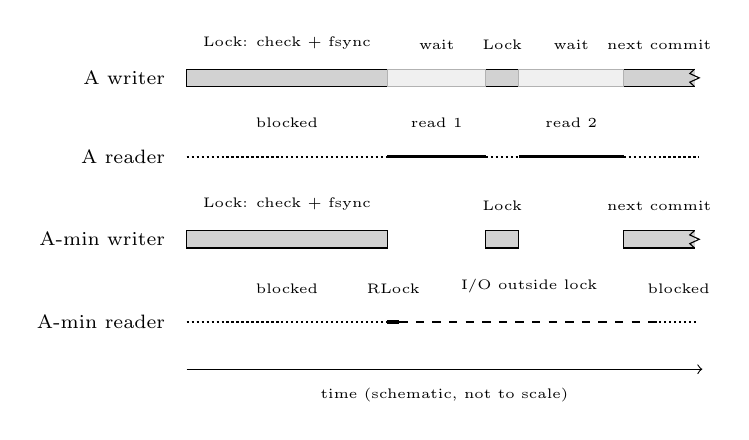
\begin{tikzpicture}[x=1cm,y=1cm,font=\scriptsize]
% Four aligned lanes; the right-hand zigzag marks the cut-off next commit.
\node[anchor=east] at (-0.15,3.8) {A writer};
\node[anchor=east] at (-0.15,2.8) {A reader};
\node[anchor=east] at (-0.15,1.75) {A-min writer};
\node[anchor=east] at (-0.15,0.7) {A-min reader};
\foreach \y in {3.8,1.75}{
 \filldraw[fill=gray!35] (0,\y-0.11) rectangle (2.55,\y+0.11);
 \node[font=\tiny,anchor=south] at (1.275,\y+0.24) {Lock: check + fsync};
 \filldraw[fill=gray!35] (3.8,\y-0.11) rectangle (4.22,\y+0.11);
 \node[font=\tiny,anchor=south] at (4.01,\y+0.24) {Lock};
 \fill[gray!35] (5.55,\y-0.11) rectangle (6.45,\y+0.11);
 \draw (6.45,\y+0.11)--(5.55,\y+0.11)--(5.55,\y-0.11)--(6.45,\y-0.11);
 \draw (6.45,\y-0.11)--(6.39,\y-0.055)--(6.51,\y)--(6.39,\y+0.055)--(6.45,\y+0.11);
 \node[font=\tiny,anchor=south] at (6.0,\y+0.24) {next commit};
}
% A's exclusive acquisitions wait until each lock-held reader interval ends.
\foreach \xa/\xb in {2.55/3.8,4.22/5.55}{
 \filldraw[draw=gray!60,fill=gray!12] (\xa,3.69) rectangle (\xb,3.91);
 \node[font=\tiny,anchor=south] at ({(\xa+\xb)/2},4.04) {wait};
}
\draw[densely dotted,thick] (0,2.8)--(2.55,2.8);
\node[font=\tiny,anchor=south] at (1.275,3.04) {blocked};
\draw[line width=1.2pt] (2.55,2.8)--(3.8,2.8);
\node[font=\tiny,anchor=south] at (3.175,3.04) {read 1};
\draw[densely dotted,thick] (3.8,2.8)--(4.22,2.8);
\draw[line width=1.2pt] (4.22,2.8)--(5.55,2.8);
\node[font=\tiny,anchor=south] at (4.885,3.04) {read 2};
\draw[densely dotted,thick] (5.55,2.8)--(6.5,2.8);
% A-min's short RLock ends before its I/O, which overruns the second Lock.
\draw[densely dotted,thick] (0,0.7)--(2.55,0.7);
\node[font=\tiny,anchor=south] at (1.275,0.94) {blocked};
\draw[line width=1.4pt] (2.55,0.7)--(2.7,0.7);
\node[font=\tiny,anchor=south] at (2.625,0.94) {RLock};
\draw[dashed,thick] (2.7,0.7)--(6.0,0.7);
\node[font=\tiny,anchor=south] at (4.35,0.94) {I/O outside lock};
\draw[densely dotted,thick] (6.0,0.7)--(6.5,0.7);
\node[font=\tiny,anchor=south] at (6.25,0.94) {blocked};
\draw[->] (0,0.1)--(6.55,0.1);
\node[font=\tiny,anchor=north] at (3.275,-0.02) {time (schematic, not to scale)};
\end{tikzpicture}
\caption{One commit cycle under A and A-min (schematic, not a measured trace). Under A the writer waits for each read and each reader completes one read per exclusive acquisition. Under A-min the reader's I/O is outside the lock and can outlast the short second acquisition. A: two reads per commit; A-min: fewer.}
\label{fig:timeline}
\end{figure}

\section{Experimental Design}
\subsection{Host, workload, and controlled dose}
The host was an AMD Ryzen 7 7445HS (6 cores, 12 logical CPUs), 15.2~GiB RAM, and Samsung MZVL8512HFLU NVMe SSD, running Windows 11 Home build 26200 on NTFS. The runner used Go 1.26.3 and \texttt{GOMAXPROCS=12}. AC power, the Best performance overlay on the Balanced base plan, and enabled Defender real-time protection were retained. Timing used QueryPerformanceCounter.

Each fixture had 10,000 keys in four SSTables of 2,500 disjoint-range keys, with 128-byte values. Reads were uniform with target hit ratio 0.95. Workers were closed-loop. Trials had 2~s warmup, a 10~s measurement window, and 200~ms cooldown. WAL fsync was enabled during measurement, disabled during fixture construction; synchronization instrumentation was enabled in all arms.

The 17 cells were X1: $r\in\{4,16\}$ crossed with $d=0$, 20~$\mu$s, 200~$\mu$s, 2~ms, and legacy (ten cells), one free-running writer and a 1~MiB memtable; X2: $r=16$, $d=0$, 200~$\mu$s, 2~ms, or legacy (four cells), no writer and twenty pre-frozen memtables released for physical publication every 0.5~s from 0.25 to 9.75~s; X3: $r\in\{1,4,16\}$, $d=0$, one writer and a 16~KiB memtable (three cells). Legacy used the retained scan without added delay.

Delay ran immediately before each point-read \texttt{ReadAt}, including conflict-validation reads. Sub-millisecond doses used a CPU-yielding spin; 2~ms used sleep then spin for the final 0.5~ms. The earlier single-goroutine probe measured approximately 9~$\mu$s, 35~$\mu$s, 215~$\mu$s, and 2.25~ms per read. These probe costs differed from concurrent lock holds, reported separately.

\subsection{Pairing, scope, and analysis}
The protocol was frozen in git before the first non-smoke trial. Ten triplets per cell paired A, A-min, and B on the same seed and operation-index request streams; completion-dependent stream prefixes could differ. Seeds used the first eight SHA-256 bytes of decimal master seed 20261030, cell ID, and triplet index separated by vertical bars, interpreted as a big-endian signed integer. Ten rounds randomized cell order using master seed plus round; arm order cycled through all six permutations. Three same-seed anchor triplets ran at the start, after round five, and at the end: 510 cell trials plus nine anchors.

$W$ and $R$ counted only in-window write and read completions. Latency histograms recorded all in-window completions without sample drops; late completions were separate. Synchronization counters reset at window start and included post-window drain, excluding fixture construction and warmup. Flush diagnostics also included drain and were not strictly in-window counts.

H1 used a one-sided exact Page trend test~\cite{page1963} on $S=W_A/W_{\mathrm{A\text{-}min}}$ across non-legacy doses, blocking by triplet index. H2 used TOST~\cite{schuirmann1987} on paired $\ln(\mathrm{A\text{-}min}/B)$, 90\% paired-$t$ CIs, margin $\pm\ln(1/0.90)$ (ratio $[0.90,1.11]$, rounded), and Holm correction~\cite{holm1979} separately for W (ten cells), R (fourteen), and publication lock-wait p99 (four). Adjusted $p<0.05$ established equivalence; a CI wholly beyond a margin meant not equivalent; otherwise the result was inconclusive. H3 used two-sided 95\% paired-$t$ CIs without a directional prediction. Descriptive ratios had 95\% CIs. Percentile bootstrap sensitivity used 10,000 resamples, seed 20261030. Cells were not pooled. The planned write-zero adjustment was never needed.

\begin{figure*}[t]
\centering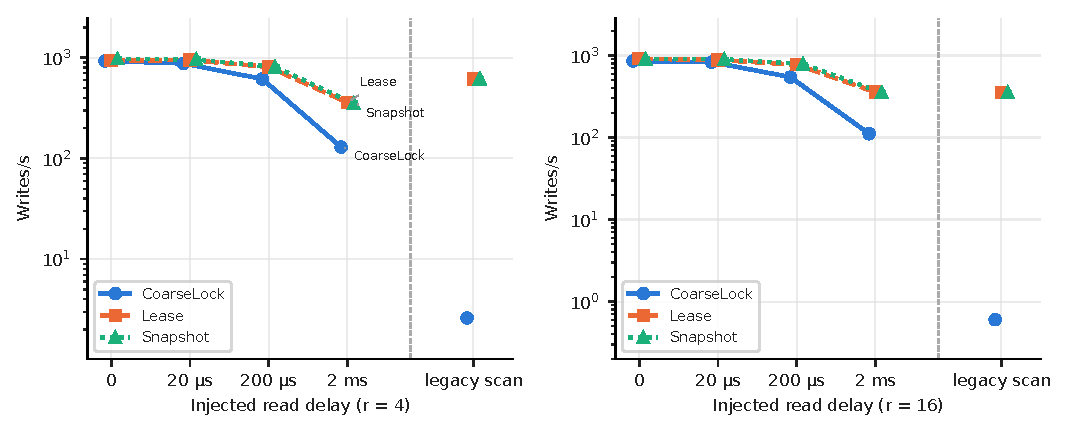
\includegraphics[width=0.90\textwidth]{fig_x1_writes.pdf}
\caption{X1 writes, $n=10$ triplets per cell. Points are per-arm geometric means; bars are 95\% $t$ CIs on log throughput, exponentiated. Most intervals are smaller than the markers. Legacy is an isolated category.}
\label{fig:writes}
\end{figure*}

\section{Results}
\subsection{RQ1: dose-response}
All 519 trials succeeded on the first attempt: no retries, exclusions, or zero adjustments. Execution ran on 2026-11-02, 12:41--14:35 UTC, about 1~h 54~min. Table~\ref{tab:x1} reports rates, paired ratios, and A's measured critical sections; Fig.~\ref{fig:writes} shows writes. All pairwise ratios with 95\% CIs for every cell are in the analysis output in the repository.

At both reader counts, Page's $L=294$, exact one-sided $p=\HOneP$, $n=10$. Geometric write ratios $S$ at 0, 20~$\mu$s, 200~$\mu$s, and 2~ms were 0.988, 0.926, 0.758, 0.361 at $r=4$, and 0.937, 0.944, 0.705, 0.311 at $r=16$. Legacy ratios were 0.0042 and 0.0017. The trend did not distinguish every adjacent dose: at $r=16$, zero and 20~$\mu$s had mean ranks 3.4 and 3.6, with no descriptive separation established between them.

Mean A read critical sections were 13.6, 33.6, 163~$\mu$s, 1.89~ms, and 125~ms (legacy) at $r=4$; at $r=16$: 21.2, 39.3, 173~$\mu$s, 1.91~ms, and 430~ms. A-min and B cell means stayed between 1.5 and 4.9~$\mu$s throughout X1. Nominal dose was not interchangeable with measured lock hold.

\begin{table*}[t]
\caption{X1, ten triplets per cell. Rates: geometric means (operations/s). CS: arithmetic mean of A's trial mean read critical sections ($\mu$s). Paired ratios have 95\% $t$ CIs.}
\label{tab:x1}\centering\scriptsize\setlength{\tabcolsep}{2.5pt}
\begin{tabular}{rrr rrr l rrr l}\toprule
 & Nominal & A CS & \multicolumn{3}{c}{Writes/s} & $S=W_A/W_{\mathrm{A\text{-}min}}$ & \multicolumn{3}{c}{Reads/s} & $R_A/R_{\mathrm{A\text{-}min}}$\\
$r$ & $d$ & $\mu$s & A & A-min & B & [95\% CI] & A & A-min & B & [95\% CI]\\\midrule
\TblXOneRows
\bottomrule\end{tabular}
\end{table*}

Read throughput showed an unpredicted result (Fig.~\ref{fig:reads}). At nominal $d=0$, 20~$\mu$s, 200~$\mu$s, and 2~ms, A/A-min read ratios were 1.193, 1.452, 1.187, and 0.725 at $r=4$, and 1.097, 1.432, 1.093, and 0.625 at $r=16$. Legacy ratios were 0.489 and 0.522, respectively. A completed more reads than A-min and B through 200~$\mu$s, crossing over between 200~$\mu$s and 2~ms. At low injected cost, coarse locking gave higher read throughput at a modest write cost in this engine and workload; by 200~$\mu$s the write cost was larger. This read-side pattern was descriptive, neither predicted nor a pre-registered test.

\begin{figure*}[t]
\centering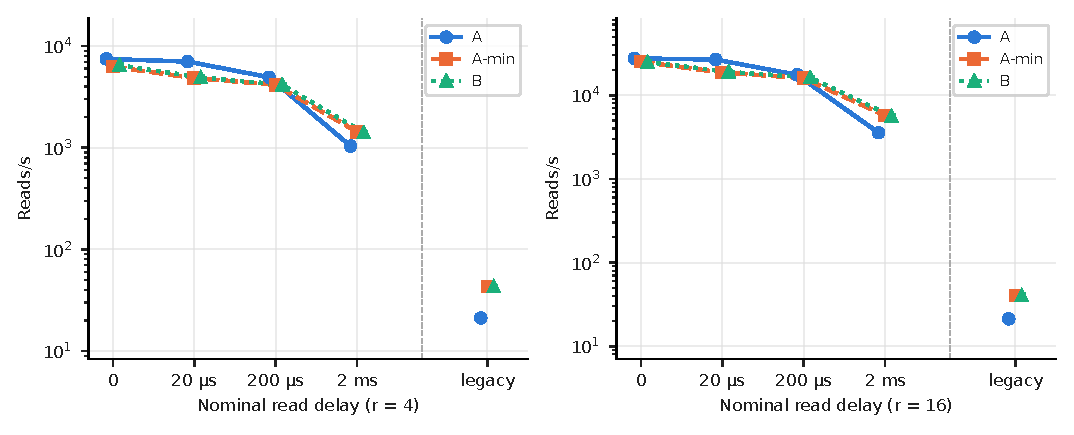
\includegraphics[width=0.90\textwidth]{fig_x1_reads.pdf}
\caption{X1 reads, $n=10$ triplets per cell. Points are geometric means; bars are exponentiated 95\% log-$t$ CIs. A's low-dose read advantage was unpredicted.}
\label{fig:reads}
\end{figure*}

\subsection{Lock-admission mechanism (exploratory, post hoc)}
Post-data source review identified two exclusive acquisitions per commit. Go's RWMutex blocks new readers behind a waiting writer and releases queued readers on unlock~\cite{goRWMutex}. With a writer continually waiting, this admission alternates reader and writer phases and resembles the phase-fair behaviour described by Brandenburg and Anderson~\cite{brandenburg2009}; we did not formally characterize it here. Under A, a reader holds the lock through its read, completing it before the next exclusive acquisition can finish. With a free-running writer and approximately one read per reader admission, this predicts
\begin{equation}R_A\simeq2rW_A.\label{eq:coupling}\end{equation}
Across ten trials in each of eleven non-legacy X1/X3 cells, individual ratios $R/(rW)$ ranged from 2.002 to 2.015. Legacy ratios ranged from 1.98 to 2.29, with only about 26 commits per trial at $r=4$ and six at $r=16$. Non-legacy coupling stayed approximately unchanged with dose or reader count.

A-min and B cell mean ratios fell from about 1.7 at zero delay to about 1.3 at 20 and 200~$\mu$s, about 1.0 at 2~ms, and 0.007--0.018 in legacy (Table~\ref{tab:mechanism}). Their I/O occurred outside the lock, so the writer's short second acquisition did not wait for it. A reader still doing I/O could miss that admission and block behind the next commit. This was consistent with the counters and Fig.~\ref{fig:timeline}, but was not tested by intervention.

A descriptive commit-cycle check used $T=1/W$ and A's measured mean first-acquisition wait $w_A$:
\begin{equation}\widehat T_A=T_{\mathrm{A\text{-}min}}+2w_A.\label{eq:cycle}\end{equation}
We averaged per-trial cycles, not reciprocals of aggregate rates. Table~\ref{tab:mechanism} gives all ten X1 comparisons. Prediction error $(\widehat T_A/T_A-1)$ ranged from $-13.8\%$ to $+10.6\%$. Only the first wait was instrumented, so an equal second wait was assumed. This was a ten-cell consistency check, not a validated model.

\begin{table*}[t]
\caption{Exploratory mechanism: arithmetic means over ten trials per cell. $q=\text{in-window reads}/(r\,\text{in-window commits})$. Cycles are ms; error is $100(\widehat T/T-1)$. X3 reports admission ratios only.}
\label{tab:mechanism}\centering\scriptsize\setlength{\tabcolsep}{5pt}
\begin{tabular}{crl rrr rrr}\toprule
Block & $r$ & Nominal $d$ & $q_A$ & $q_{\mathrm{A\text{-}min}}$ & $q_B$ & $T_A$ & $\widehat T_A$ & Error (\%)\\\midrule
\TblMechanismRows
\bottomrule\end{tabular}
\end{table*}

The dose also reached the writer: \texttt{latestValueLocked} read delayed SSTable blocks during conflict validation under exclusive \texttt{Mu} in every arm. This explained decreasing writes in A-min and B too. A-min's mean cycles at $r=4$ were 1.07, 1.06, 1.23, and 2.79~ms. The denominator of $S$ also degraded; leasing and snapshots removed only the reader's I/O hold.

Read p50 was unstable. At $r=4,d=0$, geometric mean trial p50 was 45~$\mu$s under A versus 808~$\mu$s under A-min, but p99 was 2.27 versus 2.31~ms. Reader cycles mixed a fast read with one blocked behind a roughly 1~ms commit. Bimodality was inferred from percentiles and counters; no full histogram was reported. Throughput and p99 were more informative than p50 alone.

\subsection{RQ2: A-min versus B}
All ten X1 write cells and fourteen X1/X2 read cells met H2 equivalence after Holm correction (Fig.~\ref{fig:equivalence}). All corresponding bootstrap intervals lay inside the same margin, agreeing with the throughput classifications; no bootstrap TOST replaced the planned test. Equivalence did not imply identity: X2 at $d=0$ had read ratio 0.970, 90\% CI $[0.962,0.978]$, a detectable roughly 3\% difference inside the margin.

Publication lock-wait p99 did not establish equivalence (Table~\ref{tab:h2pub}). At $d=0$, A-min/B was 3.11, 90\% CI $[1.54,6.30]$, classified not equivalent; the other cells were inconclusive. Cell geometric mean p99 waits were below 42~$\mu$s for both arms. A p99 over twenty events was close to the maximum, making this outcome noisy. Throughput equivalence did not extend to publication lock wait.

\begin{table}[t]
\caption{H2 publication lock-wait p99, $n=10$ triplets: paired ratio, 90\% $t$ CI, and planned classification.}
\label{tab:h2pub}\centering\scriptsize\setlength{\tabcolsep}{3pt}
\begin{tabular}{lll}\toprule
Nominal $d$ & A-min/B [90\% CI] & Class\\\midrule
\TblHTwoPubRows
\bottomrule\end{tabular}
\end{table}

\subsection{X2: publication}
At zero delay, 200~$\mu$s, and 2~ms, every arm published 20/20 tables within the window in every trial (Table~\ref{tab:x2}, Fig.~\ref{fig:publication}). In legacy, A's median was 10.5, range 9--11; A-min and B completed 20/20 throughout. Publication deadline failure therefore appeared only at legacy in this setting. A's geometric mean publication lock-wait p99 was 247~$\mu$s, 450~$\mu$s, 3.89~ms, and 1.05~s (legacy arithmetic mean 1.06~s). At zero delay, A-min and B were 41.6 and 13.4~$\mu$s. X2 A/A-min read ratios were 1.05, 1.00, 1.00, and 0.65.

\begin{figure*}[t]
\centering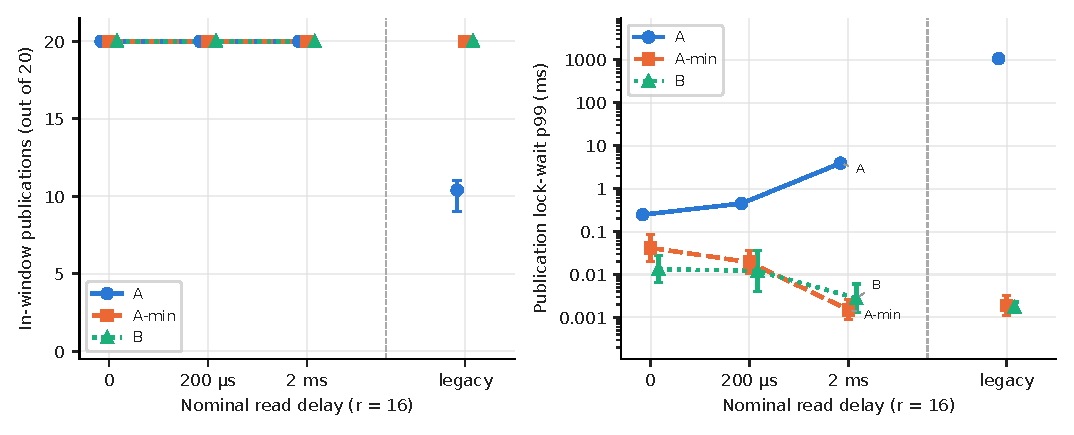
\includegraphics[width=0.90\textwidth]{fig_x2_publication.pdf}
\caption{X2, $n=10$ triplets per cell. Left: arithmetic mean in-window count, min--max bars. Right: geometric mean trial publication lock-wait p99, exponentiated 95\% log-$t$ CIs. Wait instrumentation included drain.}
\label{fig:publication}
\end{figure*}

\begin{table*}[t]
\caption{X2, ten triplets: geometric mean read rate and trial lock-wait p99 ($\mu$s); in-window publications are median [min, max], out of twenty.}
\label{tab:x2}\centering\scriptsize\setlength{\tabcolsep}{4pt}
\begin{tabular}{l rrr lll rrr}\toprule
Nominal & \multicolumn{3}{c}{Reads/s} & \multicolumn{3}{c}{In-window publications} & \multicolumn{3}{c}{Lock-wait p99 ($\mu$s)}\\
$d$ & A & A-min & B & A & A-min & B & A & A-min & B\\\midrule
\TblXTwoRows
\bottomrule\end{tabular}
\end{table*}

\subsection{RQ3: churn}
With 16~KiB memtables, mean measured flush counts ranged from 38.8 to 73.2 per trial (10~s window plus drain). Table~\ref{tab:x3} reports rates and both interval methods. A-min/B read ratios at $r=1,4,16$ were 0.956, 1.005, 0.970; write ratios were 0.957, 1.004, 0.968. All 95\% paired-$t$ CIs included one. Bootstrap intervals at $r=1$ and $r=16$ narrowly excluded one for both outcomes, e.g., $[0.909,0.997]$ for reads at $r=1$. Small differences favoring B could not be ruled out.

A/B read ratios were 1.66, 1.53, 1.29; write ratios were 0.89, 0.84, 0.71. The read deficit relative to A also occurred in A-min at the same size. A-min did not allocate reader-set snapshot descriptors, so these data did not support attributing the deficit to snapshot lifecycle cost or claiming A-min avoided a churn penalty. This was consistent with admission ratios near 2.01 under A and about 1.1 under both alternatives.

\begin{figure*}[t]
\centering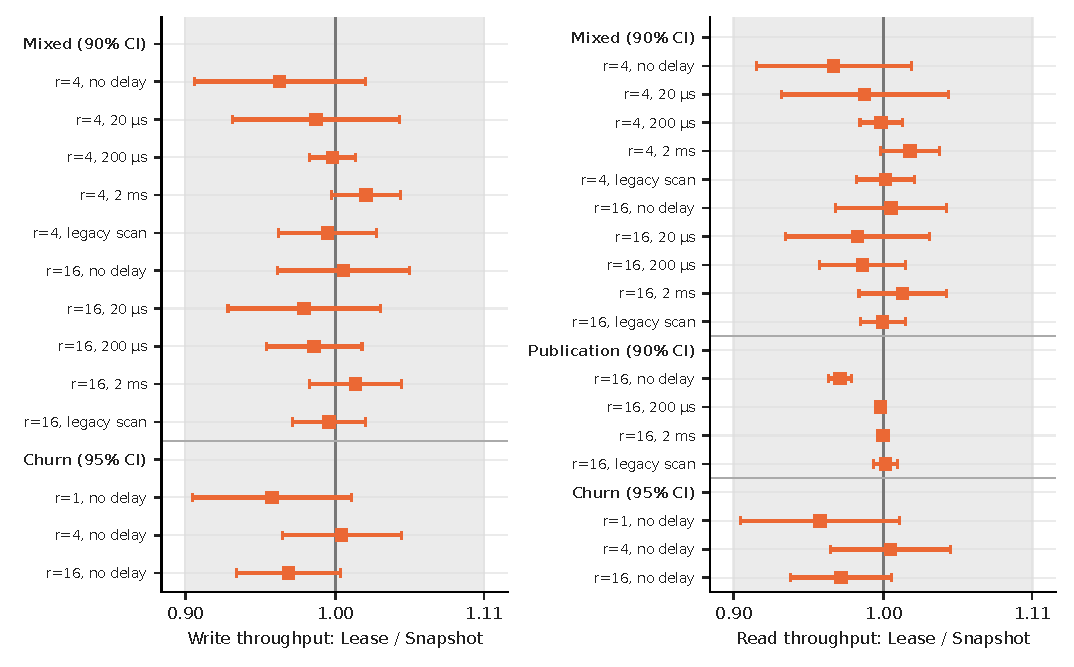
\includegraphics[width=0.90\textwidth]{fig_amin_vs_b.pdf}
\caption{A-min/B throughput, $n=10$ triplets per cell. Points: paired geometric ratios; bars: exponentiated paired log-$t$ CIs, 90\% in X1/X2 and 95\% in X3. Shading: rounded H2 margin $[0.90,1.11]$. X3 was not an equivalence test.}
\label{fig:equivalence}
\end{figure*}

\begin{table*}[t]
\caption{X3, ten triplets per cell. Arm rates: geometric means (operations/s). A-min/B: 95\% paired-$t$ CI and 95\% percentile bootstrap CI. Flushes: arithmetic means for A/A-min/B, including drain.}
\label{tab:x3}\centering\scriptsize\setlength{\tabcolsep}{5pt}
\begin{tabular}{rc rrr lll}\toprule
$r$ & Outcome & A & A-min & B & A-min/B [95\% $t$ CI] & Bootstrap CI & Flushes A/A-min/B\\\midrule
\TblXThreeRows
\bottomrule\end{tabular}
\end{table*}

Pre-registered anchor drift was $D=R_{\mathrm{A\text{-}min}}(t10)/R_{\mathrm{A\text{-}min}}(t00)=\DriftD$, $|\ln D|=\DriftLog$, below the 0.10 threat threshold. For transparency, A and B end/start ratios were both about 1.09, log ratios 0.087 and 0.090: below, but near, that threshold. Each anchor arm/time was a single trial.

\begin{figure}[t]
\centering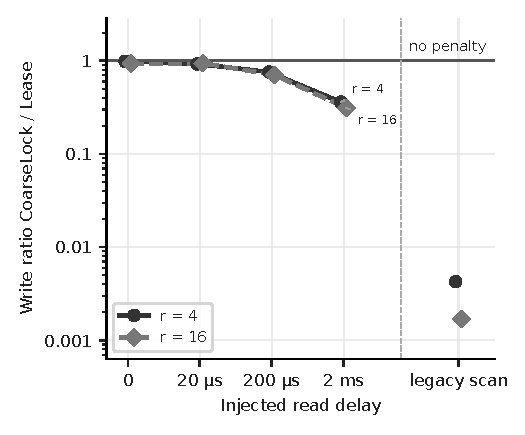
\includegraphics[width=0.96\columnwidth]{fig_x1_ratio.pdf}
\caption{X1 write ratio A/A-min, $n=10$ triplets per cell. Points: paired geometric means; bars: exponentiated 95\% paired log-$t$ CIs.}
\label{fig:ratio}
\end{figure}

\section{Discussion}
The write penalty grew as A's shared critical section lengthened and was small at tens of microseconds. Its low-cost read advantage showed that admission policy and exclusive acquisitions per commit could determine read throughput more than critical-section length alone. File lifetime and admission frequency should be evaluated together.

Leasing matched snapshots within the declared throughput margin in X1/X2. This established no advantage of A-min over B and removed neither exclusive conflict validation nor fsync. Churn did not isolate descriptor allocation as the cause of A's read advantage. Publication wait required a separate conclusion from throughput.

Implications for this class of engine are conditional. Measure lock-held read duration before replacing a coarse lock: here, at tested holds below about 40~$\mu$s, point-estimate write penalties were within 8\%, and A completed more reads. At nominal 20~$\mu$s, however, the 95\% CIs for $S$ were $[0.881,0.974]$ at $r=4$ and $[0.887,1.004]$ at $r=16$; 8\% was not a confidence bound. At tested holds above about 150~$\mu$s, point-estimate penalties were at least 24\%. Shorter reader holds left the writer's exclusive work, which set the A-min/B commit cycle; a writer-side change may be the next step. Admission policy can be part of the performance model. These implications do not establish transfer to other engines.

Future work should remove the second acquisition, for example by an atomic size check, and test the coupling by intervention. Moving fsync and conflict validation out of the exclusive lock, group commit, other lock policies, larger datasets, and multiple writers would test the account's boundaries. Such changes require correctness validation as well as performance measurement.

\section{Threats to Validity}
Injected delay was a controlled proxy, not a device model. Every visited point-read SSTable block incurred delay without application block-cache hits. Sub-millisecond delays spun while yielding; sixteen readers exceeded twelve logical CPUs, so CPU contention was part of those cells. The 10,000-key dataset was likely in the OS page cache. Uniform, closed-loop access and one writer restricted workload scope.

WAL fsync remained under the exclusive lock without group commit, setting an approximately 1~ms commit floor in low-cost cells. LevelDB releases its mutex during log writing and synchronization~\cite{leveldb}; results do not transfer directly to engines with group commit. The optional WAL-sync-off run was not performed; the X harness rejected \texttt{wal\_sync=false}. Two acquisitions and Go's policy were engine-specific: Eq.~\ref{eq:coupling} should not be generalized.

The mechanism and read-side interpretation were post hoc. The protocol's statement that A-min and B did not hold the lock across delay applied to readers only; delayed writer conflict checks were noticed after collection. The cycle model assumed an unmeasured second wait, and bimodality was inferred without reporting a full histogram. One laptop, OS, and file system, with Defender enabled, limited external validity.

An operator stopped the first start at 38 of 519 trials for power-supply reasons unrelated to results. It was discarded unanalysed; only status lines were seen. A 21-trial smoke run was seen before analysis rules were fixed and was excluded; no design value changed because of it. Fixtures were built without fsync. Race detection passed on Linux under WSL2 with Go 1.27.3, not on Windows. The author was sole experimenter and analyst; there was no independent replication.

\section{Related Work}
The LSM-tree~\cite{oneil1996lsm} and survey~\cite{luo2020} frame the storage organization. LevelDB and RocksDB~\cite{leveldb,rocksdb} provide reference implementations; Dong et al.~\cite{dong2021} describe RocksDB's evolving development priorities. Our arms do not reproduce their production designs or workloads. Golan-Gueta et al.~\cite{golan2015} propose cLSM, an algorithm for scalable concurrency in LSM data stores. SILK~\cite{balmau2019} addresses latency spikes in LSM stores.

Courtois et al.~\cite{courtois1971} pose the readers--writers problem, Mellor-Crummey and Scott~\cite{mellor1991} give scalable reader-writer algorithms, and Brandenburg and Anderson~\cite{brandenburg2009} propose phase-fair locks. Go's RWMutex documentation~\cite{goRWMutex} supplies the policy here. Page's ordered-rank test~\cite{page1963}, Schuirmann's TOST~\cite{schuirmann1987}, and Holm's correction~\cite{holm1979} supplied the pre-registered methods.

\section{Conclusion}
Across the completed 519-trial campaign, coarse read locking's write penalty increased with measured critical-section length and was small at tens of microseconds. A nevertheless completed more reads than A-min and B through nominal 200~$\mu$s. Exploratory counters were consistent with two reader admissions per commit under A, suggesting that lock policy and exclusive-acquisition count shaped the low-cost regime. Leasing matched snapshots within the declared throughput margin in all ten X1 write and fourteen X1/X2 read cells; publication lock-wait equivalence was not established. Neither removed the writer's exclusive work. Churn did not isolate snapshot lifecycle cost. These findings are bounded by this engine, host, and workload.

\section*{Data Availability}
Source, plan, frozen protocol, analysis and figure scripts are in \url{https://github.com/itsramhere/selfdbms}, branch \texttt{research/x-readcost}; trial records are archived with the repository. The measured revision was \texttt{c53ee5b}. Plan SHA-256 began \texttt{68ad96f878c1}; runner SHA-256 began \texttt{22060ffc4885}. Tables came from final results and trial envelopes via \texttt{x\_readcost\_paper\_tables.py}. A claim-to-evidence map is at \texttt{paper/CLAIM\_EVIDENCE\_MAP\_X.md}.

\begin{thebibliography}{15}
\bibitem{oneil1996lsm} P. O'Neil, E. Cheng, D. Gawlick, and E. O'Neil, ``The log-structured merge-tree (LSM-tree),'' \emph{Acta Informatica}, vol. 33, no. 4, pp. 351--385, 1996.
\bibitem{leveldb} S. Ghemawat and J. Dean, ``LevelDB,'' GitHub repository google/leveldb. [Online]. Available: \url{https://github.com/google/leveldb}
\bibitem{rocksdb} Meta Platforms, ``RocksDB,'' GitHub repository facebook/rocksdb. [Online]. Available: \url{https://github.com/facebook/rocksdb}
\bibitem{dong2021} S. Dong, A. Kryczka, Y. Jin, and M. Stumm, ``RocksDB: Evolution of development priorities in a key-value store serving large-scale applications,'' \emph{ACM Trans. Storage}, vol. 17, no. 4, Art. 26, 2021.
\bibitem{luo2020} C. Luo and M. J. Carey, ``LSM-based storage techniques: a survey,'' \emph{The VLDB Journal}, vol. 29, no. 1, pp. 393--418, 2020.
\bibitem{golan2015} G. Golan-Gueta, E. Bortnikov, E. Hillel, and I. Keidar, ``Scaling concurrent log-structured data stores,'' in \emph{Proc. EuroSys}, 2015, Art. 32.
\bibitem{balmau2019} O. Balmau, F. Dinu, W. Zwaenepoel, K. Gupta, R. Chandhiramoorthi, and D. Didona, ``SILK: Preventing latency spikes in log-structured merge key-value stores,'' in \emph{Proc. USENIX ATC}, 2019, pp. 753--766.
\bibitem{courtois1971} P. J. Courtois, F. Heymans, and D. L. Parnas, ``Concurrent control with `readers' and `writers','' \emph{Commun. ACM}, vol. 14, no. 10, pp. 667--668, 1971.
\bibitem{mellor1991} J. M. Mellor-Crummey and M. L. Scott, ``Scalable reader-writer synchronization for shared-memory multiprocessors,'' in \emph{Proc. PPoPP}, 1991, pp. 106--113.
\bibitem{brandenburg2009} B. B. Brandenburg and J. H. Anderson, ``Reader-writer synchronization for shared-memory multiprocessor real-time systems,'' in \emph{Proc. ECRTS}, 2009, pp. 184--193.
\bibitem{pugh1990} W. Pugh, ``Skip lists: A probabilistic alternative to balanced trees,'' \emph{Commun. ACM}, vol. 33, no. 6, pp. 668--676, 1990.
\bibitem{goRWMutex} The Go Authors, ``sync package: RWMutex.'' [Online]. Available: \url{https://pkg.go.dev/sync#RWMutex}
\bibitem{page1963} E. B. Page, ``Ordered hypotheses for multiple treatments: A significance test for linear ranks,'' \emph{J. Amer. Statist. Assoc.}, vol. 58, no. 301, pp. 216--230, 1963.
\bibitem{schuirmann1987} D. J. Schuirmann, ``A comparison of the two one-sided tests procedure and the power approach for assessing the equivalence of average bioavailability,'' \emph{J. Pharmacokinet. Biopharm.}, vol. 15, no. 6, pp. 657--680, 1987.
\bibitem{holm1979} S. Holm, ``A simple sequentially rejective multiple test procedure,'' \emph{Scand. J. Statist.}, vol. 6, no. 2, pp. 65--70, 1979.
\end{thebibliography}
\end{document}
